% Choose one to switch betweeen slides and handout
%\documentclass[]{beamer}
\documentclass[handout]{beamer}

% Video Meta Data
\title{Bitcoin, Blockchain and Cryptoassets}
\subtitle{Economic Scripting}
\author{Prof. Dr. Fabian Schär}
\institute{University of Basel}

% Config File
% Packages
\usepackage[utf8]{inputenc}
\usepackage{hyperref}
\usepackage{gitinfo2}
\usepackage{tikz}
\usepackage{amsmath}
\usepackage{bibentry}
\usepackage{xcolor}
\usepackage{colortbl} % Add colour to LaTeX tables
\usepackage{caption}
\usepackage[export]{adjustbox}
\usepackage{pgfplots} \pgfplotsset{compat = 1.17}

% Color Options
\definecolor{highlight}{rgb}{0.65,0.84,0.82}
\definecolor{focus}{rgb}{0.72, 0, 0}

% Beamer Template Options
\beamertemplatenavigationsymbolsempty
\setbeamertemplate{footline}[frame number]
\setbeamercolor{structure}{fg=black}
\setbeamercolor{footline}{fg=black}
\setbeamercolor{title}{fg=black}
\setbeamercolor{frametitle}{fg=black}
\setbeamercolor{item}{fg=black}
\setbeamercolor{}{fg=black}
\setbeamercolor{bibliography item}{fg=black}
\setbeamercolor*{bibliography entry title}{fg=black}
\setbeamertemplate{items}[square]
\setbeamertemplate{enumerate items}[default]
\captionsetup[figure]{labelfont={color=black},font={color=black}}
\captionsetup[table]{labelfont={color=black},font={color=black}}

\setbeamertemplate{bibliography item}{\insertbiblabel}

% Link Icon Command
\newcommand{\link}{%
    \tikz[x=1.2ex, y=1.2ex, baseline=-0.05ex]{%
        \begin{scope}[x=1ex, y=1ex]
            \clip (-0.1,-0.1)
                --++ (-0, 1.2)
                --++ (0.6, 0)
                --++ (0, -0.6)
                --++ (0.6, 0)
                --++ (0, -1);
            \path[draw,
                line width = 0.5,
                rounded corners=0.5]
                (0,0) rectangle (1,1);
        \end{scope}
        \path[draw, line width = 0.5] (0.5, 0.5)
            -- (1, 1);
        \path[draw, line width = 0.5] (0.6, 1)
            -- (1, 1) -- (1, 0.6);
        }
    }

% Read Git Data from Github Actions Workflow
% Defaults to gitinfo2 for local builds
\IfFileExists{gitInfo.txt}
	{\input{gitInfo.txt}}
	{
		\newcommand{\gitRelease}{(Local Release)}
		\newcommand{\gitSHA}{\gitHash}
		\newcommand{\gitDate}{\gitAuthorIsoDate}
	}

% Custom Titlepage
\defbeamertemplate*{title page}{customized}[1][]
{
  \vspace{-0cm}\hfill
\includegraphics[width=2.5cm]{../config/logo_cif}
  
\includegraphics[width=1.9cm]{../config/seal_wwz}
  \\ \vspace{2em}
  \usebeamerfont{title}\textbf{\inserttitle}\par
  \usebeamerfont{title}\usebeamercolor[fg]{title}\insertsubtitle\par  \vspace{1.5em}
  \small\usebeamerfont{author}\insertauthor\par
  \usebeamerfont{author}\insertinstitute\par \vspace{2em}
  \usebeamercolor[fg]{titlegraphic}\inserttitlegraphic
    \tiny \noindent \texttt{Release Ver.: \gitRelease}\\ 
    \texttt{Version Hash: \gitSHA}\\
    \texttt{Version Date: \gitDate}\\ \vspace{1em}
  \link \href{https://github.com/cifunibas/Bitcoin-Blockchain-Cryptoassets/blob/main/slides/intro.pdf}
  {Get most recent version}\\
  \link \href{https://github.com/cifunibas/Bitcoin-Blockchain-Cryptoassets/blob/main/slides/intro.pdf}
  {Watch video lecture}\\ \vspace{1em}
  License: \texttt{Creative Commons Attribution-NonCommercial-ShareAlike 4.0 International}\\\vspace{2em}
  
\includegraphics[width = 1.2cm]{../config/license}
}

% tikzlibraries
\usetikzlibrary{decorations.pathreplacing}
\usetikzlibrary{decorations.markings}
\usetikzlibrary{positioning}

%caption font
\captionsetup{font=footnotesize}


% Other Inputs
% Defining Bitcoin Symbol
\def\btc{%
	\leavevmode
	\vtop{\offinterlineskip %\bfseries
		\setbox0=\hbox{B}%
		\setbox2=\hbox to\wd0{\hfil\hskip-.03em
			\vrule height .3ex width .15ex\hskip .08em
			\vrule height .3ex width .15ex\hfil}
		\vbox{\copy2\box0}\box2}}
% Definition of a green checkmark symbol
% Code based on: https://tex.stackexchange.com/questions/532033/make-a-double-blue-checkmark-symbol-with-square-contours-using-tikz

% Create shape of a green checkmark
\tikzset{pics/.cd, checkmark/.style={code={% 
			\pgfgettransformentries{\tmpxx}{\tmp}{\tmp}{\tmp}{\tmp}{\tmp}
			\draw[line width=\tmpxx*1pt,draw=none,fill=green!60] (0,.33) -- (.25,0) to 
			(0.8,.6) to (.72,.68) to (.25,.18) to (0.08,.40)-- cycle;}}}

\newcommand{\checkmarkgreen}{
\begin{tikzpicture}[baseline={(0,0)}]
		\path (0,0) pic[scale=1]{checkmark};
\end{tikzpicture}}



%%%%%%%%%%%%%%%%%%%%%%%%%%%%%%%%%%%%%%%%%%%%%%
%%%%%%%%%%%%%%%%%%%%%%%%%%%%%%%%%%%%%%%%%%%%%%
\begin{document}

\thispagestyle{empty}
\begin{frame}[noframenumbering]
	\titlepage
\end{frame}

%%%

\begin{frame}{Transactions Review}
	What has been covered so far:
	\begin{itemize}
		\item<1 -> Transaction types
		\begin{itemize}
			\item<1 -> Pay-to-Address, Pay-to-Multisig, Pay-to-Script-Hash, etc.
		\end{itemize}
		\item<2 -> Signature hash types
		\begin{itemize}
			\item<2 -> \texttt{SIGHASH\_ALL}, \texttt{SIGHASH\_NONE|SIGHASH\_ANYONECANPAY}, etc.
		\end{itemize}
		\item<3 -> Using these components and clever transaction design smart contracts can be implemented on the Bitcoin Blockchain
	\end{itemize}
\end{frame}

%%%

\begin{frame}{Example: Conditional Purchase Agreement}
	\begin{figure}[h]
		\begin{minipage}{0.2\linewidth}
			\centering
			
\includegraphics[width=1cm]{../assets/images/agents/handing_right}
			\begin{tikzpicture}[overlay]
				\node at (-0.05,0.18) {
\includegraphics[width = 0.5cm]{../assets/images/bitcoin}};
			\end{tikzpicture}
		\end{minipage}%
		\begin{minipage}{0.15\linewidth}
			\centering
			\vspace{-2cm}
			\only<3>{
\includegraphics[width=1cm]{../assets/images/agents/intermediary_devil}}
		\end{minipage}%
		\begin{minipage}{0.25\linewidth}
			\centering
			
\includegraphics[width=1cm]{../assets/images/agents/handing_left}
			\begin{tikzpicture}[overlay, coloredCoin/.style={circle,  very thick, minimum size=0.5mm}]
				\node[coloredCoin, draw=orange!60, fill=orange!5] at (-1.5,0.9) {\footnotesize{$\btc$}};
			\end{tikzpicture}
		\end{minipage}
	\end{figure}
	\begin{itemize}
		\item<1 ->Story: Alice wants to purchase a colored coin from Bob
		\item<2 ->Issue: None of the two wants to transfer their asset first
		\item<3 ->Traditionally, centralized service would be used 
		\item<4 ->Using an elegant transaction design, they can do the transaction on-chain and trustless
	\end{itemize}
\end{frame}

%%%

\begin{frame}{Example: Conditional Purchase Agreement}
	\begin{figure}
			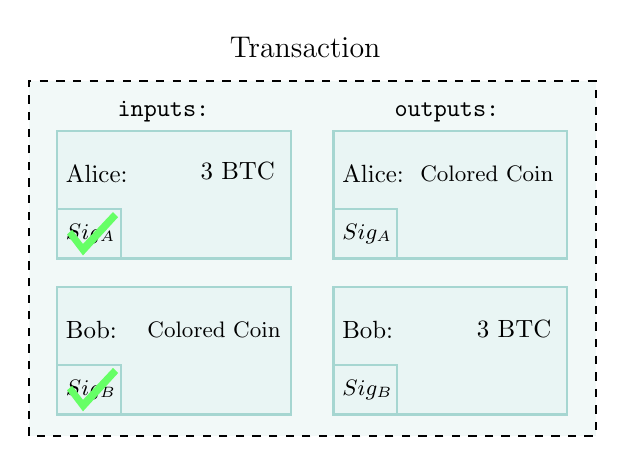
\begin{tikzpicture}[scale=0.9, every node/.style={scale=0.9}]
				\filldraw[yshift=-0.05cm, xshift=0.1cm,color = highlight!15, thick, 	draw=black, dashed] (-3,-5.9) rectangle ++(8cm,5cm);
				
				\draw[color=black] plot (1,-0.2) node [below]
				{\large{{Transaction}}};
				
				% Inputs
				\draw[color=black] plot (-1,-1.65) node[above] {\texttt{inputs:}};
				
				% top left
				\filldraw[yshift=-0.05cm, xshift=0.1cm,color = highlight!25, thick, 	draw=highlight] (-2.6,-3.4) rectangle ++(3.3cm,1.8cm);
				\filldraw[yshift=-0.05cm, xshift=0.1cm,color = highlight!25, thick, 	draw=highlight] (-2.6,-3.4) rectangle ++(0.9cm,0.7cm);
				\draw[color=black] plot (-2.5,-2.25) node[right] {Alice:};
				\draw[color=black] plot (-0.6,-2.21)   node[right] {3 BTC};
				\draw[color=black] plot (-2.5,-3.1)   node[right] {\small{$Sig_A$}};
			
				\uncover<2 ->{\draw plot (-2,-3.1) node {\checkmarkgreen};}
						
				% bottom left
				\uncover<3->{
				\filldraw[yshift=-0.05cm, xshift=0.1cm,color = highlight!25, thick, draw=highlight] (-2.6,-5.6) rectangle ++(3.3cm,1.8cm);
				\filldraw[yshift=-0.05cm, xshift=0.1cm,color = highlight!25, thick,draw=highlight] (-2.6,-5.6) rectangle ++(0.9cm,0.7cm);
				\draw[color=black] plot (-2.5,-4.45)   node[right] {Bob:};
				\draw[color=black] plot (-1.35,-4.45)   node[right] {\small{Colored Coin}};
				\draw[color=black] plot (-2.5,-5.3)   node[right] {\small{$Sig_B$}};}
				
				\uncover<4->{\draw plot (-2,-5.3) node {\checkmarkgreen};}
				
				% Outputs
				\draw[color=black] plot (3,-1.65)   node[above] {\texttt{outputs:}};
				
				% top right
				\filldraw[yshift=-0.05cm, xshift=0.1cm,color = highlight!25, thick, draw=highlight] (1.3,-3.4) rectangle ++(3.3cm,1.8cm);
				\filldraw[yshift=-0.05cm, xshift=0.1cm,color = highlight!25, thick, 	draw=highlight] (1.3,-3.4) rectangle ++(0.9cm,0.7cm);
				\draw[color=black] plot (1.4,-2.25)   node[right] {Alice:};
				\draw[color=black] plot (2.5,-2.25)   node[right] {\small{Colored Coin}};
				\draw[color=black] plot (1.4,-3.1)   node[right] {\small{$Sig_A$}};
				
				% bottom right
				\filldraw[yshift=-0.05cm, xshift=0.1cm,color = highlight!25, thick, draw=highlight] (1.3,-5.6) rectangle ++(3.3cm,1.8cm);
				\filldraw[yshift=-0.05cm, xshift=0.1cm,color = highlight!25, thick,draw=highlight] (1.3,-5.6) rectangle ++(0.9cm,0.7cm);
				\draw[color=black] plot (1.4,-4.45)   node[right] {Bob:};
				\draw[color=black] plot (3.3,-4.45)   node[right] {3 BTC};
				\draw[color=black] plot (1.4,-5.3)   node[right] {\small{$Sig_B$}};
		\end{tikzpicture}
	\end{figure}
	\begin{itemize}
		\item<1 ->Alice creates "wrapper" transaction (SIGHASH\_ALL) and signes her input
		\item<3 ->Bob signes his input
		\item<4 ->Transfers executed simultaneously. No counterparty risk.
	\end{itemize}
\end{frame}

%%%

\begin{frame}{Time Locks}
	\begin{itemize}
		\item<1-> UTXOs can be locked for a specified time
		\begin{itemize}
			\item<1-> Absolute time locks use a specific point in time or block height (analogy: "at 12 o'clock")
			\item<1-> Relative time locks specify a number of blocks after confirmation (analogy: "in five hours")
		\end{itemize}
		\item<2 -> Four alternatives for implementation
	\end{itemize}
	\vspace{0.25cm}
	\uncover<2->{\begin{table}
		\center
		\resizebox{\textwidth}{!}{%
			\begin{tabular}{lll} \hline \hline
				& Transaction level     & Output level\\
				\cline{2-3}
				& Consensus             & Scripting Language\\ \hline
				Absolute time lock  & \texttt{nLockTime}    & CHECKLOCKTIMEVERIFY (CLTV)\\ 
				Relative time lock  & \texttt{nSequence}    & CHECKSEQUENCEVERIFY (CSV)\\\hline \hline
		\end{tabular}}
	\end{table}}
\end{frame}

%%%
\iffalse
\begin{frame}{Example: Simple Payment Channel}
	\begin{itemize}
		\item<1 ->Alice wants to pay Bob many small transaction without paying to much in transaction fees or spaming the network
		\item<2 ->She opens a unidirectional payment channel
		\begin{itemize}
			\item<2 ->Payment channels allow parties to exchange transactions off-chain, while still benefiting from the security of the Bitcoin Blockchain
		\end{itemize}\vspace{0.2cm}
		\item<3 ->Off-chain preparation:
		\begin{itemize}
			\item<3 ->Alice opens a 2-of-2 multisig address
			\item<4 ->Alice creates a \textit{funding transaction} to the multisig address
			\item<5 ->Next, she creates a \textit{refund transaction} from the multisig address back to her address and lets Bob sign and return this transaction
			\item<6 ->The \textit{refund transaction} contains a \texttt{nLockTime} time lock and guarantees that all remaining funds on the multisig are returned to Alice after specified period of time
		\end{itemize}\vspace{0.2cm}
		\item<7 ->On-chain transaction:
		\begin{itemize}
			\item<7 ->Alice propagates the \textit{funding transaction}
		\end{itemize}
	\end{itemize}
\end{frame}
\fi
%%%

\begin{frame}{Example: Simple Payment Channel}
	\begin{minipage}{0.1\linewidth}
		\vspace{-0.5cm}
		\centering
		
\includegraphics[width=1cm]{../assets/images/agents/handing_right}
		\\ \hspace{-0.35cm} \textbf{Alice}
	\end{minipage}%
	\begin{minipage}{0.8\linewidth}
		\begin{figure}
		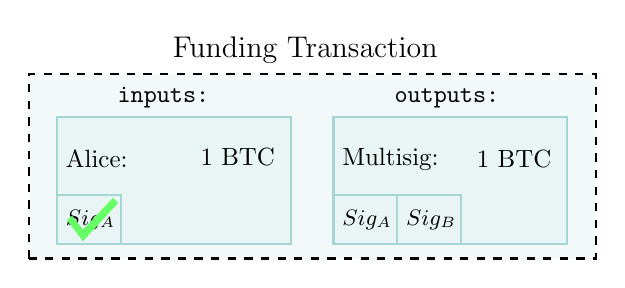
\begin{tikzpicture}[scale=0.9, every node/.style={scale=0.9}]
			
	\filldraw[yshift=-0.05cm, xshift=0.1cm,color = highlight!15, thick, 	draw=black, dashed] (-3,-3.6) rectangle ++(8cm,2.6cm);
	
	\draw[color=black] plot (1,-0.4) node [below]
	{\large{{Funding Transaction}}};
	
	% Inputs
	\draw[color=black] plot (-1,-1.65) node[above] {\texttt{inputs:}};
	
	% top left
	\filldraw[yshift=-0.05cm, xshift=0.1cm,color = highlight!25, thick, 	draw=highlight] (-2.6,-3.4) rectangle ++(3.3cm,1.8cm);
	\filldraw[yshift=-0.05cm, xshift=0.1cm,color = highlight!25, thick, 	draw=highlight] (-2.6,-3.4) rectangle ++(0.9cm,0.7cm);
	\draw[color=black] plot (-2.5,-2.25) node[right] {Alice:};
	\draw[color=black] plot (-0.6,-2.21)   node[right] {1 BTC};
	\draw[color=black] plot (-2.5,-3.1)   node[right] {\small{$Sig_A$}};
	
	\draw plot (-2,-3.1) node {\checkmarkgreen};
	
	% Outputs
	\draw[color=black] plot (3,-1.65)   node[above] {\texttt{outputs:}};
	
	% top right
	\filldraw[yshift=-0.05cm, xshift=0.1cm,color = highlight!25, thick, draw=highlight] (1.3,-3.4) rectangle ++(3.3cm,1.8cm);
	\filldraw[yshift=-0.05cm, xshift=0.1cm,color = highlight!25, thick, 	draw=highlight] (1.3,-3.4) rectangle ++(0.9cm,0.7cm);
	\filldraw[yshift=-0.05cm, xshift=0.1cm,color = highlight!25, thick, 	draw=highlight] (2.2,-3.4) rectangle ++(0.9cm,0.7cm);
	\draw[color=black] plot (1.4,-2.25)   node[right] {Multisig:};
	\draw[color=black] plot (3.3,-2.25)   node[right] {1 BTC};
	\draw[color=black] plot (1.4,-3.1)   node[right] {\small{$Sig_A$}};
	\draw[color=black] plot (2.3,-3.1)   node[right] {\small{$Sig_B$}};

		\end{tikzpicture}
		\vspace{0.5cm}
		\uncover<2 ->{
		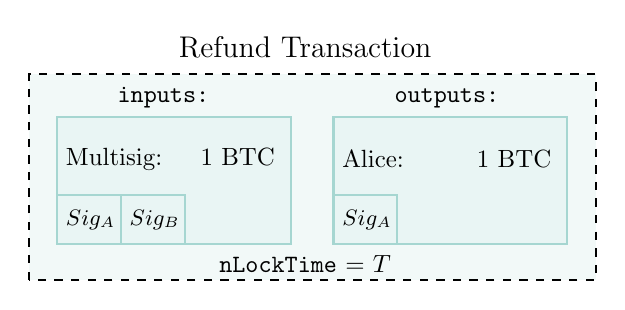
\begin{tikzpicture}[scale=0.9, every node/.style={scale=0.9}]
				\filldraw[yshift=-0.05cm, xshift=0.1cm,color = highlight!15, thick, 	draw=black, dashed] (-3,-3.9) rectangle ++(8cm,2.9cm);
	
	\draw[color=black] plot (1,-0.4) node [below]
	{\large{{Refund Transaction}}};
	
	% Inputs
	\draw[color=black] plot (-1,-1.65) node[above] {\texttt{inputs:}};
	
	% top left
	\filldraw[yshift=-0.05cm, xshift=0.1cm,color = highlight!25, thick, 	draw=highlight] (-2.6,-3.4) rectangle ++(3.3cm,1.8cm);
	\filldraw[yshift=-0.05cm, xshift=0.1cm,color = highlight!25, thick, 	draw=highlight] (-2.6,-3.4) rectangle 	++(0.9cm,0.7cm);
	\filldraw[yshift=-0.05cm, xshift=0.1cm,color = highlight!25, thick, 	draw=highlight] (-1.7,-3.4) rectangle 	++(0.9cm,0.7cm);
	\draw[color=black] plot (-2.5,-2.25) node[right] {Multisig:};
	\draw[color=black] plot (-0.6,-2.21)   node[right] {1 BTC};
	\draw[color=black] plot (-2.5,-3.1)   node[right] {\small{$Sig_A$}};
	\draw[color=black] plot (-1.6,-3.1)   node[right] {\small{$Sig_B$}};
	
	% Outputs
	\draw[color=black] plot (3,-1.65)   node[above] {\texttt{outputs:}};
	
	% top right
	\filldraw[yshift=-0.05cm, xshift=0.1cm,color = highlight!25, thick, draw=highlight] (1.3,-3.4) rectangle ++(3.3cm,1.8cm);
	\filldraw[yshift=-0.05cm, xshift=0.1cm,color = highlight!25, thick, 	draw=highlight] (1.3,-3.4) rectangle ++(0.9cm,0.7cm);
	\draw[color=black] plot (1.4,-2.25)   node[right] {Alice:};
	\draw[color=black] plot (3.3,-2.25)   node[right] {1 BTC};
	\draw[color=black] plot (1.4,-3.1)   node[right] {\small{$Sig_A$}};
	
	% Time lock
	\draw[color=black] plot (1,-3.97)   node[above] {\texttt{nLockTime} = $T$};

		\end{tikzpicture}
		}
		\end{figure}
	\end{minipage}%
	\begin{minipage}{0.1\linewidth}
		\vspace{-0.5cm}
		\centering
		
\includegraphics[width=1cm]{../assets/images/agents/handing_left}
		\\ \hspace{0.3cm}\textbf{Bob}
	\end{minipage}
\end{frame}

%%%

\begin{frame}{Example: Simple Payment Channel}
	\begin{minipage}{0.1\linewidth}
		\vspace{-2.1cm}
		\begin{figure}[t]
			\resizebox{2.5cm}{!}{
			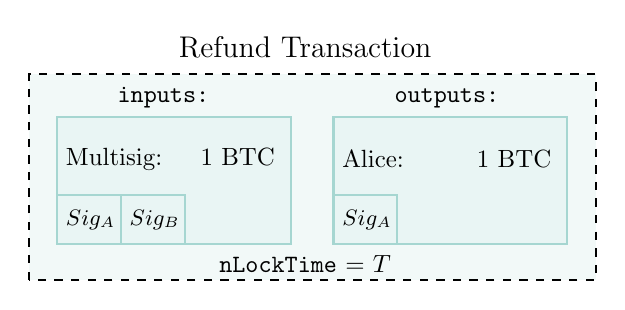
\begin{tikzpicture}[scale=0.9, every node/.style={scale=0.9}]
						\filldraw[yshift=-0.05cm, xshift=0.1cm,color = highlight!15, thick, 	draw=black, dashed] (-3,-3.9) rectangle ++(8cm,2.9cm);
	
	\draw[color=black] plot (1,-0.4) node [below]
	{\large{{Refund Transaction}}};
	
	% Inputs
	\draw[color=black] plot (-1,-1.65) node[above] {\texttt{inputs:}};
	
	% top left
	\filldraw[yshift=-0.05cm, xshift=0.1cm,color = highlight!25, thick, 	draw=highlight] (-2.6,-3.4) rectangle ++(3.3cm,1.8cm);
	\filldraw[yshift=-0.05cm, xshift=0.1cm,color = highlight!25, thick, 	draw=highlight] (-2.6,-3.4) rectangle 	++(0.9cm,0.7cm);
	\filldraw[yshift=-0.05cm, xshift=0.1cm,color = highlight!25, thick, 	draw=highlight] (-1.7,-3.4) rectangle 	++(0.9cm,0.7cm);
	\draw[color=black] plot (-2.5,-2.25) node[right] {Multisig:};
	\draw[color=black] plot (-0.6,-2.21)   node[right] {1 BTC};
	\draw[color=black] plot (-2.5,-3.1)   node[right] {\small{$Sig_A$}};
	\draw[color=black] plot (-1.6,-3.1)   node[right] {\small{$Sig_B$}};
	
	% Outputs
	\draw[color=black] plot (3,-1.65)   node[above] {\texttt{outputs:}};
	
	% top right
	\filldraw[yshift=-0.05cm, xshift=0.1cm,color = highlight!25, thick, draw=highlight] (1.3,-3.4) rectangle ++(3.3cm,1.8cm);
	\filldraw[yshift=-0.05cm, xshift=0.1cm,color = highlight!25, thick, 	draw=highlight] (1.3,-3.4) rectangle ++(0.9cm,0.7cm);
	\draw[color=black] plot (1.4,-2.25)   node[right] {Alice:};
	\draw[color=black] plot (3.3,-2.25)   node[right] {1 BTC};
	\draw[color=black] plot (1.4,-3.1)   node[right] {\small{$Sig_A$}};
	
	% Time lock
	\draw[color=black] plot (1,-3.97)   node[above] {\texttt{nLockTime} = $T$};

			\end{tikzpicture}}
		\end{figure}
		\centering
		
\includegraphics[width=1cm]{../assets/images/agents/handing_right}
		\\ \hspace{-0.35cm} \textbf{Alice}
	\end{minipage}%
	\begin{minipage}{0.8\linewidth}
		\uncover<3->{
		\vspace{1cm}
		\begin{figure}
				\resizebox{5cm}{!}{
					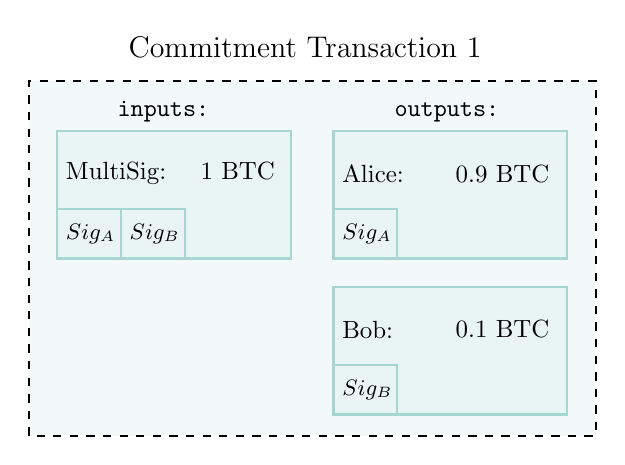
\begin{tikzpicture}[scale=0.9, every node/.style={scale=0.9}]
							\filldraw[yshift=-0.05cm, xshift=0.1cm,color = highlight!15, thick, 	draw=black, dashed] (-3,-5.9) rectangle ++(8cm,5cm);
	
	\draw[color=black] plot (1,-0.2) node [below]
	{\large{{Commitment Transaction 1}}};
	
	% Inputs
	\draw[color=black] plot (-1,-1.65) node[above] {\texttt{inputs:}};
	
	% top left
	\filldraw[yshift=-0.05cm, xshift=0.1cm,color = highlight!25, thick, 	draw=highlight] (-2.6,-3.4) rectangle ++(3.3cm,1.8cm);
	\filldraw[yshift=-0.05cm, xshift=0.1cm,color = highlight!25, thick, 	draw=highlight] (-2.6,-3.4) rectangle ++(0.9cm,0.7cm);
	\filldraw[yshift=-0.05cm, xshift=0.1cm,color = highlight!25, thick, 	draw=highlight] (-1.7,-3.4) rectangle ++(0.9cm,0.7cm);
	\draw[color=black] plot (-2.5,-2.25) node[right] {MultiSig:};
	\draw[color=black] plot (-0.6,-2.21)   node[right] {1 BTC};
	\draw[color=black] plot (-2.5,-3.1)   node[right] {\small{$Sig_A$}};
	\draw[color=black] plot (-1.6,-3.1)   node[right] {\small{$Sig_B$}};
	
	% Outputs
	\draw[color=black] plot (3,-1.65)   node[above] {\texttt{outputs:}};
	
	% top right
	\filldraw[yshift=-0.05cm, xshift=0.1cm,color = highlight!25, thick, draw=highlight] (1.3,-3.4) rectangle ++(3.3cm,1.8cm);
	\filldraw[yshift=-0.05cm, xshift=0.1cm,color = highlight!25, thick, 	draw=highlight] (1.3,-3.4) rectangle ++(0.9cm,0.7cm);
	\draw[color=black] plot (1.4,-2.25)   node[right] {Alice:};
	\draw[color=black] plot (3,-2.25)   node[right] {0.9 BTC};
	\draw[color=black] plot (1.4,-3.1)   node[right] {\small{$Sig_A$}};
	
	% bottom right
	\filldraw[yshift=-0.05cm, xshift=0.1cm,color = highlight!25, thick, draw=highlight] (1.3,-5.6) rectangle ++(3.3cm,1.8cm);
	\filldraw[yshift=-0.05cm, xshift=0.1cm,color = highlight!25, thick,draw=highlight] (1.3,-5.6) rectangle ++(0.9cm,0.7cm);
	\draw[color=black] plot (1.4,-4.45)   node[right] {Bob:};
	\draw[color=black] plot (3,-4.45)   node[right] {0.1 BTC};
	\draw[color=black] plot (1.4,-5.3)   node[right] {\small{$Sig_B$}};

				\end{tikzpicture}}
		\end{figure}}
		\begin{figure}
			\centering
			\resizebox{4cm}{!}{
			\begin{tikzpicture}[scale=1, every node/.style={scale=1}]
					
% Title
%\node[above] at (2,4.3) {Peer-to-Peer};


% Network
\node (agenta) at (1,2.8) {
\includegraphics[width = 0.6 cm]{../assets/images/agents/avatar_rand3.png}};
\node (agentb) at (0.5,1) {
\includegraphics[width = 0.6 cm]{../assets/images/agents/avatar_rand4.png}};
\node (agentc) at (3,2.1) {
\includegraphics[width = 0.6 cm]{../assets/images/agents/avatar_rand5.png}};
\node (agentd) at (2.8,0) {
\includegraphics[width = 0.6 cm]{../assets/images/agents/avatar_rand1.png}};
\node (agente) at (5,4.3) {
\includegraphics[width = 0.6 cm]{../assets/images/agents/avatar_rand2.png}};	
\node (agentf) at (5.1,1.1) {
\includegraphics[width = 0.6 cm]{../assets/images/agents/avatar_rand3.png}};
\node (agentg) at (7.5,3.8) {
\includegraphics[width = 0.6 cm]{../assets/images/agents/avatar_rand4.png}};
\node (agenth) at (6.7,0.4) {
\includegraphics[width = 0.6 cm]{../assets/images/agents/avatar_rand5.png}};

% Network flow
\draw[<->, thick, dashed]	(agenta.south) -- (agentb.north);
\draw[<->, thick, dashed] 	(agenta.east) -- (agente.west);
\draw[<->, thick, dashed]	(agenta.south east) -- (agentc.west);
\draw[<->, thick, dashed]	(agente.south west) -- (agentc.north east);
\draw[<->, thick, dashed]	(agente.south) -- (agentf.north);
\draw[<->, thick, dashed]	(agente.east) -- (agentg.west);
\draw[<->, thick, dashed]	(agentc.south west) -- (agentb.east);
\draw[<->, thick, dashed]	(agentc.south) -- (agentd.north);
\draw[<->, thick, dashed]	(agentc.south east) --  (agentf.west);
\draw[<->, thick, dashed]	(agentg.south west) -- (agentf.north east);
\draw[<->, thick, dashed]	(agentg.south) -- (agenth.north);
\draw[<->, thick, dashed]	(agentb.south east) -- (agentd.west);
\draw[<->, thick, dashed]	(agentf.south west) -- (agentd.east);
\draw[<->, thick, dashed]	(agentf.south east) -- (agenth.west);
\draw[<->, thick, dashed]	(agenth.south west) -- (agentd.east);

			\end{tikzpicture}}
		\end{figure}
		\uncover<2>{
			\vspace{-2.6cm}
			\begin{figure}
				\resizebox{2.5cm}{!}{
				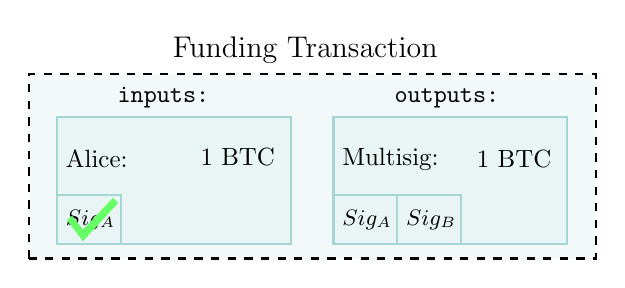
\begin{tikzpicture}[scale=0.9, every node/.style={scale=0.9}]
						
	\filldraw[yshift=-0.05cm, xshift=0.1cm,color = highlight!15, thick, 	draw=black, dashed] (-3,-3.6) rectangle ++(8cm,2.6cm);
	
	\draw[color=black] plot (1,-0.4) node [below]
	{\large{{Funding Transaction}}};
	
	% Inputs
	\draw[color=black] plot (-1,-1.65) node[above] {\texttt{inputs:}};
	
	% top left
	\filldraw[yshift=-0.05cm, xshift=0.1cm,color = highlight!25, thick, 	draw=highlight] (-2.6,-3.4) rectangle ++(3.3cm,1.8cm);
	\filldraw[yshift=-0.05cm, xshift=0.1cm,color = highlight!25, thick, 	draw=highlight] (-2.6,-3.4) rectangle ++(0.9cm,0.7cm);
	\draw[color=black] plot (-2.5,-2.25) node[right] {Alice:};
	\draw[color=black] plot (-0.6,-2.21)   node[right] {1 BTC};
	\draw[color=black] plot (-2.5,-3.1)   node[right] {\small{$Sig_A$}};
	
	\draw plot (-2,-3.1) node {\checkmarkgreen};
	
	% Outputs
	\draw[color=black] plot (3,-1.65)   node[above] {\texttt{outputs:}};
	
	% top right
	\filldraw[yshift=-0.05cm, xshift=0.1cm,color = highlight!25, thick, draw=highlight] (1.3,-3.4) rectangle ++(3.3cm,1.8cm);
	\filldraw[yshift=-0.05cm, xshift=0.1cm,color = highlight!25, thick, 	draw=highlight] (1.3,-3.4) rectangle ++(0.9cm,0.7cm);
	\filldraw[yshift=-0.05cm, xshift=0.1cm,color = highlight!25, thick, 	draw=highlight] (2.2,-3.4) rectangle ++(0.9cm,0.7cm);
	\draw[color=black] plot (1.4,-2.25)   node[right] {Multisig:};
	\draw[color=black] plot (3.3,-2.25)   node[right] {1 BTC};
	\draw[color=black] plot (1.4,-3.1)   node[right] {\small{$Sig_A$}};
	\draw[color=black] plot (2.3,-3.1)   node[right] {\small{$Sig_B$}};

				\end{tikzpicture}}
			\end{figure}
		}		
	\end{minipage}%
	\begin{minipage}{0.1\linewidth}
		\vspace{-0.5cm}
		\centering
		
\includegraphics[width=1cm]{../assets/images/agents/handing_left}
		\\ \hspace{0.3cm}\textbf{Bob}
	\end{minipage}
\end{frame}

%%%

\begin{frame}{Example: Simple Payment Channel}
	\begin{minipage}{0.1\linewidth}
		\vspace{-2.27cm}
		\begin{figure}[t]
			\resizebox{2.5cm}{!}{
			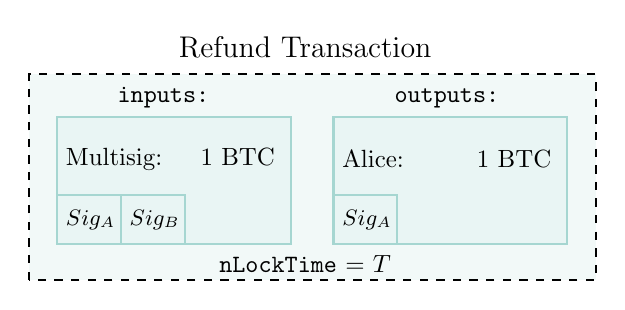
\begin{tikzpicture}[scale=0.9, every node/.style={scale=0.9}]
					\filldraw[yshift=-0.05cm, xshift=0.1cm,color = highlight!15, thick, 	draw=black, dashed] (-3,-3.9) rectangle ++(8cm,2.9cm);
	
	\draw[color=black] plot (1,-0.4) node [below]
	{\large{{Refund Transaction}}};
	
	% Inputs
	\draw[color=black] plot (-1,-1.65) node[above] {\texttt{inputs:}};
	
	% top left
	\filldraw[yshift=-0.05cm, xshift=0.1cm,color = highlight!25, thick, 	draw=highlight] (-2.6,-3.4) rectangle ++(3.3cm,1.8cm);
	\filldraw[yshift=-0.05cm, xshift=0.1cm,color = highlight!25, thick, 	draw=highlight] (-2.6,-3.4) rectangle 	++(0.9cm,0.7cm);
	\filldraw[yshift=-0.05cm, xshift=0.1cm,color = highlight!25, thick, 	draw=highlight] (-1.7,-3.4) rectangle 	++(0.9cm,0.7cm);
	\draw[color=black] plot (-2.5,-2.25) node[right] {Multisig:};
	\draw[color=black] plot (-0.6,-2.21)   node[right] {1 BTC};
	\draw[color=black] plot (-2.5,-3.1)   node[right] {\small{$Sig_A$}};
	\draw[color=black] plot (-1.6,-3.1)   node[right] {\small{$Sig_B$}};
	
	% Outputs
	\draw[color=black] plot (3,-1.65)   node[above] {\texttt{outputs:}};
	
	% top right
	\filldraw[yshift=-0.05cm, xshift=0.1cm,color = highlight!25, thick, draw=highlight] (1.3,-3.4) rectangle ++(3.3cm,1.8cm);
	\filldraw[yshift=-0.05cm, xshift=0.1cm,color = highlight!25, thick, 	draw=highlight] (1.3,-3.4) rectangle ++(0.9cm,0.7cm);
	\draw[color=black] plot (1.4,-2.25)   node[right] {Alice:};
	\draw[color=black] plot (3.3,-2.25)   node[right] {1 BTC};
	\draw[color=black] plot (1.4,-3.1)   node[right] {\small{$Sig_A$}};
	
	% Time lock
	\draw[color=black] plot (1,-3.97)   node[above] {\texttt{nLockTime} = $T$};

			\end{tikzpicture}}
		\end{figure}
		\centering
		
\includegraphics[width=1cm]{../assets/images/agents/handing_right}
		\\ \hspace{-0.35cm} \textbf{Alice}
	\end{minipage}%
	\begin{minipage}{0.8\linewidth}
		\vspace{1.34cm}
		\only<1>{
			\begin{figure}
				\resizebox{5cm}{!}{
					\begin{tikzpicture}
						\filldraw[yshift=-0.05cm, xshift=0.1cm,color = white!15, thick, draw=white] (-3,-5.9) rectangle ++(8cm,5.7cm);
				\end{tikzpicture}}
		\end{figure}}
		\only<2-3>{
			\begin{figure}
				\resizebox{5cm}{!}{
				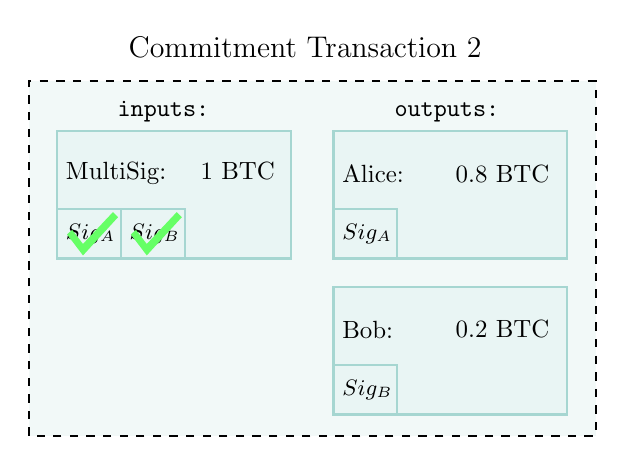
\begin{tikzpicture}[scale=0.9, every node/.style={scale=0.9}]
					\filldraw[yshift=-0.05cm, xshift=0.1cm,color = highlight!15, thick, 	draw=black, dashed] (-3,-5.9) rectangle ++(8cm,5cm);

\draw[color=black] plot (1,-0.2) node [below]
{\large{{Commitment Transaction 2}}};

% Inputs
\draw[color=black] plot (-1,-1.65) node[above] {\texttt{inputs:}};

% top left
\filldraw[yshift=-0.05cm, xshift=0.1cm,color = highlight!25, thick, 	draw=highlight] (-2.6,-3.4) rectangle ++(3.3cm,1.8cm);
\filldraw[yshift=-0.05cm, xshift=0.1cm,color = highlight!25, thick, 	draw=highlight] (-2.6,-3.4) rectangle ++(0.9cm,0.7cm);
\filldraw[yshift=-0.05cm, xshift=0.1cm,color = highlight!25, thick, 	draw=highlight] (-1.7,-3.4) rectangle ++(0.9cm,0.7cm);
\draw[color=black] plot (-2.5,-2.25) node[right] {MultiSig:};
\draw[color=black] plot (-0.6,-2.21)   node[right] {1 BTC};
\draw[color=black] plot (-2.5,-3.1)   node[right] {\small{$Sig_A$}};
\draw[color=black] plot (-1.6,-3.1)   node[right] {\small{$Sig_B$}};

\draw plot (-2,-3.1) node {\checkmarkgreen};
\uncover<3->{\draw plot (-1.1,-3.1) node {\checkmarkgreen};}

% Outputs
\draw[color=black] plot (3,-1.65)   node[above] {\texttt{outputs:}};

% top right
\filldraw[yshift=-0.05cm, xshift=0.1cm,color = highlight!25, thick, draw=highlight] (1.3,-3.4) rectangle ++(3.3cm,1.8cm);
\filldraw[yshift=-0.05cm, xshift=0.1cm,color = highlight!25, thick, 	draw=highlight] (1.3,-3.4) rectangle ++(0.9cm,0.7cm);
\draw[color=black] plot (1.4,-2.25)   node[right] {Alice:};
\draw[color=black] plot (3,-2.25)   node[right] {0.8 BTC};
\draw[color=black] plot (1.4,-3.1)   node[right] {\small{$Sig_A$}};

% bottom right
\filldraw[yshift=-0.05cm, xshift=0.1cm,color = highlight!25, thick, draw=highlight] (1.3,-5.6) rectangle ++(3.3cm,1.8cm);
\filldraw[yshift=-0.05cm, xshift=0.1cm,color = highlight!25, thick,draw=highlight] (1.3,-5.6) rectangle ++(0.9cm,0.7cm);
\draw[color=black] plot (1.4,-4.45)   node[right] {Bob:};
\draw[color=black] plot (3,-4.45)   node[right] {0.2 BTC};
\draw[color=black] plot (1.4,-5.3)   node[right] {\small{$Sig_B$}};
				\end{tikzpicture}}
		\end{figure}}
		\only<4>{
			\begin{figure}
				\resizebox{5cm}{!}{
				\begin{tikzpicture}
						\filldraw[yshift=-0.05cm, xshift=0.1cm,color = white!15, thick, draw=white] (-3,-5.9) rectangle ++(8cm,5.7cm);
				\end{tikzpicture}}
		\end{figure}}
		\begin{figure}
			\centering
			\resizebox{4cm}{!}{
				\begin{tikzpicture}[scale=1, every node/.style={scale=1}]
					
% Title
%\node[above] at (2,4.3) {Peer-to-Peer};


% Network
\node (agenta) at (1,2.8) {
\includegraphics[width = 0.6 cm]{../assets/images/agents/avatar_rand3.png}};
\node (agentb) at (0.5,1) {
\includegraphics[width = 0.6 cm]{../assets/images/agents/avatar_rand4.png}};
\node (agentc) at (3,2.1) {
\includegraphics[width = 0.6 cm]{../assets/images/agents/avatar_rand5.png}};
\node (agentd) at (2.8,0) {
\includegraphics[width = 0.6 cm]{../assets/images/agents/avatar_rand1.png}};
\node (agente) at (5,4.3) {
\includegraphics[width = 0.6 cm]{../assets/images/agents/avatar_rand2.png}};	
\node (agentf) at (5.1,1.1) {
\includegraphics[width = 0.6 cm]{../assets/images/agents/avatar_rand3.png}};
\node (agentg) at (7.5,3.8) {
\includegraphics[width = 0.6 cm]{../assets/images/agents/avatar_rand4.png}};
\node (agenth) at (6.7,0.4) {
\includegraphics[width = 0.6 cm]{../assets/images/agents/avatar_rand5.png}};

% Network flow
\draw[<->, thick, dashed]	(agenta.south) -- (agentb.north);
\draw[<->, thick, dashed] 	(agenta.east) -- (agente.west);
\draw[<->, thick, dashed]	(agenta.south east) -- (agentc.west);
\draw[<->, thick, dashed]	(agente.south west) -- (agentc.north east);
\draw[<->, thick, dashed]	(agente.south) -- (agentf.north);
\draw[<->, thick, dashed]	(agente.east) -- (agentg.west);
\draw[<->, thick, dashed]	(agentc.south west) -- (agentb.east);
\draw[<->, thick, dashed]	(agentc.south) -- (agentd.north);
\draw[<->, thick, dashed]	(agentc.south east) --  (agentf.west);
\draw[<->, thick, dashed]	(agentg.south west) -- (agentf.north east);
\draw[<->, thick, dashed]	(agentg.south) -- (agenth.north);
\draw[<->, thick, dashed]	(agentb.south east) -- (agentd.west);
\draw[<->, thick, dashed]	(agentf.south west) -- (agentd.east);
\draw[<->, thick, dashed]	(agentf.south east) -- (agenth.west);
\draw[<->, thick, dashed]	(agenth.south west) -- (agentd.east);

			\end{tikzpicture}}
		\end{figure}
		\vspace{-2.9cm}
		\uncover<4 ->{
		\begin{figure}
			\resizebox{2.5cm}{!}{
				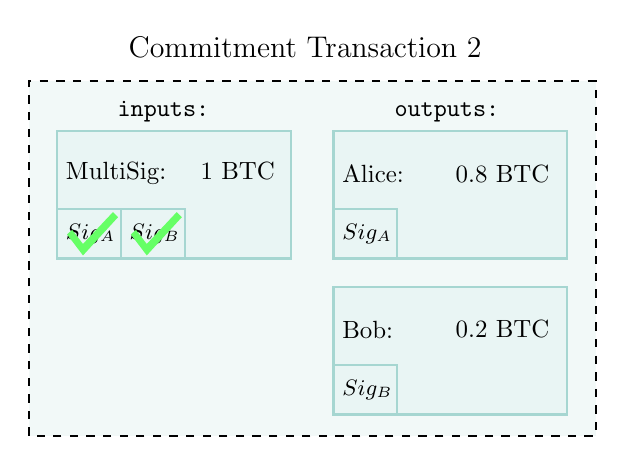
\begin{tikzpicture}[scale=0.9, every node/.style={scale=0.9}]
					\filldraw[yshift=-0.05cm, xshift=0.1cm,color = highlight!15, thick, 	draw=black, dashed] (-3,-5.9) rectangle ++(8cm,5cm);

\draw[color=black] plot (1,-0.2) node [below]
{\large{{Commitment Transaction 2}}};

% Inputs
\draw[color=black] plot (-1,-1.65) node[above] {\texttt{inputs:}};

% top left
\filldraw[yshift=-0.05cm, xshift=0.1cm,color = highlight!25, thick, 	draw=highlight] (-2.6,-3.4) rectangle ++(3.3cm,1.8cm);
\filldraw[yshift=-0.05cm, xshift=0.1cm,color = highlight!25, thick, 	draw=highlight] (-2.6,-3.4) rectangle ++(0.9cm,0.7cm);
\filldraw[yshift=-0.05cm, xshift=0.1cm,color = highlight!25, thick, 	draw=highlight] (-1.7,-3.4) rectangle ++(0.9cm,0.7cm);
\draw[color=black] plot (-2.5,-2.25) node[right] {MultiSig:};
\draw[color=black] plot (-0.6,-2.21)   node[right] {1 BTC};
\draw[color=black] plot (-2.5,-3.1)   node[right] {\small{$Sig_A$}};
\draw[color=black] plot (-1.6,-3.1)   node[right] {\small{$Sig_B$}};

\draw plot (-2,-3.1) node {\checkmarkgreen};
\uncover<3->{\draw plot (-1.1,-3.1) node {\checkmarkgreen};}

% Outputs
\draw[color=black] plot (3,-1.65)   node[above] {\texttt{outputs:}};

% top right
\filldraw[yshift=-0.05cm, xshift=0.1cm,color = highlight!25, thick, draw=highlight] (1.3,-3.4) rectangle ++(3.3cm,1.8cm);
\filldraw[yshift=-0.05cm, xshift=0.1cm,color = highlight!25, thick, 	draw=highlight] (1.3,-3.4) rectangle ++(0.9cm,0.7cm);
\draw[color=black] plot (1.4,-2.25)   node[right] {Alice:};
\draw[color=black] plot (3,-2.25)   node[right] {0.8 BTC};
\draw[color=black] plot (1.4,-3.1)   node[right] {\small{$Sig_A$}};

% bottom right
\filldraw[yshift=-0.05cm, xshift=0.1cm,color = highlight!25, thick, draw=highlight] (1.3,-5.6) rectangle ++(3.3cm,1.8cm);
\filldraw[yshift=-0.05cm, xshift=0.1cm,color = highlight!25, thick,draw=highlight] (1.3,-5.6) rectangle ++(0.9cm,0.7cm);
\draw[color=black] plot (1.4,-4.45)   node[right] {Bob:};
\draw[color=black] plot (3,-4.45)   node[right] {0.2 BTC};
\draw[color=black] plot (1.4,-5.3)   node[right] {\small{$Sig_B$}};
			\end{tikzpicture}}
		\end{figure}}		
	\end{minipage}%
	\begin{minipage}{0.1\linewidth}
		\vspace{1.44cm}
		\centering
		
\includegraphics[width=1cm]{../assets/images/agents/handing_left}
		\\ \hspace{0.3cm}\textbf{Bob}
		\vspace{-0.5cm}
		\begin{figure}
		\hspace{-1.7cm}
		\resizebox{2.5cm}{!}{
				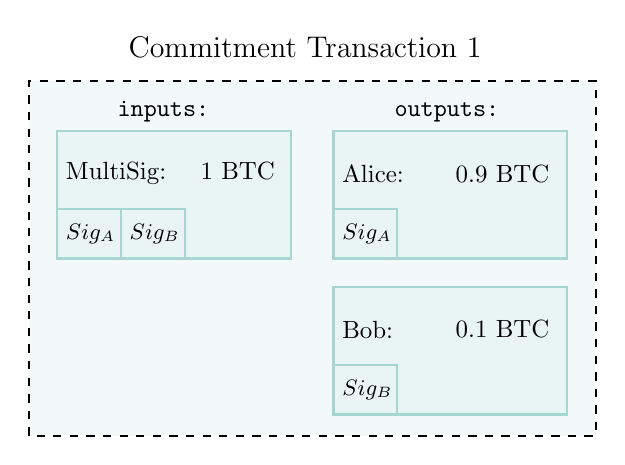
\begin{tikzpicture}[scale=0.9, every node/.style={scale=0.9}]
						\filldraw[yshift=-0.05cm, xshift=0.1cm,color = highlight!15, thick, 	draw=black, dashed] (-3,-5.9) rectangle ++(8cm,5cm);
	
	\draw[color=black] plot (1,-0.2) node [below]
	{\large{{Commitment Transaction 1}}};
	
	% Inputs
	\draw[color=black] plot (-1,-1.65) node[above] {\texttt{inputs:}};
	
	% top left
	\filldraw[yshift=-0.05cm, xshift=0.1cm,color = highlight!25, thick, 	draw=highlight] (-2.6,-3.4) rectangle ++(3.3cm,1.8cm);
	\filldraw[yshift=-0.05cm, xshift=0.1cm,color = highlight!25, thick, 	draw=highlight] (-2.6,-3.4) rectangle ++(0.9cm,0.7cm);
	\filldraw[yshift=-0.05cm, xshift=0.1cm,color = highlight!25, thick, 	draw=highlight] (-1.7,-3.4) rectangle ++(0.9cm,0.7cm);
	\draw[color=black] plot (-2.5,-2.25) node[right] {MultiSig:};
	\draw[color=black] plot (-0.6,-2.21)   node[right] {1 BTC};
	\draw[color=black] plot (-2.5,-3.1)   node[right] {\small{$Sig_A$}};
	\draw[color=black] plot (-1.6,-3.1)   node[right] {\small{$Sig_B$}};
	
	% Outputs
	\draw[color=black] plot (3,-1.65)   node[above] {\texttt{outputs:}};
	
	% top right
	\filldraw[yshift=-0.05cm, xshift=0.1cm,color = highlight!25, thick, draw=highlight] (1.3,-3.4) rectangle ++(3.3cm,1.8cm);
	\filldraw[yshift=-0.05cm, xshift=0.1cm,color = highlight!25, thick, 	draw=highlight] (1.3,-3.4) rectangle ++(0.9cm,0.7cm);
	\draw[color=black] plot (1.4,-2.25)   node[right] {Alice:};
	\draw[color=black] plot (3,-2.25)   node[right] {0.9 BTC};
	\draw[color=black] plot (1.4,-3.1)   node[right] {\small{$Sig_A$}};
	
	% bottom right
	\filldraw[yshift=-0.05cm, xshift=0.1cm,color = highlight!25, thick, draw=highlight] (1.3,-5.6) rectangle ++(3.3cm,1.8cm);
	\filldraw[yshift=-0.05cm, xshift=0.1cm,color = highlight!25, thick,draw=highlight] (1.3,-5.6) rectangle ++(0.9cm,0.7cm);
	\draw[color=black] plot (1.4,-4.45)   node[right] {Bob:};
	\draw[color=black] plot (3,-4.45)   node[right] {0.1 BTC};
	\draw[color=black] plot (1.4,-5.3)   node[right] {\small{$Sig_B$}};

				\end{tikzpicture}}
		\end{figure}
	\end{minipage}
\end{frame}

%%%

\begin{frame}{Example: Simple Payment Channel}
	\begin{table}
		\begin{tabular}{c c c c c}
			\hline
			State & Alice & Bob & Open Conditions & \texttt{nLockTime}\\
			\hline
			State 0 & 1.0 & 0.0 & $Sig_A$ & $T$\\
			State 1 & 0.9 & 0.1 & $Sig_B$ & \\
			State 2 & 0.8 & 0.2 & $Sig_B$ & \\
			\hline
		\end{tabular}
	\end{table}
	\vspace{0.2cm}
	\uncover<2 ->{
	\begin{figure}
		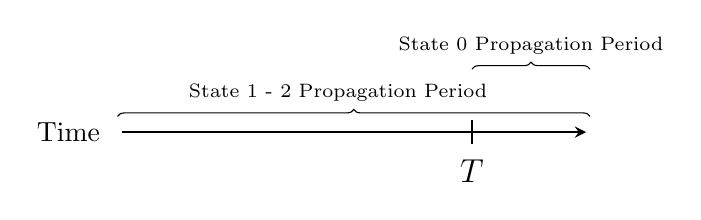
\begin{tikzpicture}
			\draw[color=black] plot (-1.1,1) node[left] {Time};
			\draw[-stealth,thick,shorten >=0.05cm,shorten <=0.05cm] (-1,1) -- (5,1);
			\draw[thick] (3.5,1.15) -- (3.5,0.85);
			\draw[color=black] plot (3.5,0.5) node {\large{$T$}};
			
			\draw[color=black] plot (1.8,1.5) node {\scriptsize{State 1 - 2 Propagation Period}};
			\draw[color=black] plot (4.25,2.1) node {\scriptsize{State 0 Propagation Period}};
			
			\draw [decoration={brace}, decorate] (-1,1.2) -- (5,1.2);
			\draw [decoration={brace}, decorate] (3.5,1.8) -- (5,1.8);
		\end{tikzpicture}
	\end{figure}}
	\vspace{0.2cm}
	\begin{itemize}
		\item<3 -> Incentive compatible: Bob will pick latest state and propagate it before $T$
	\end{itemize}
\end{frame}

%%%

%\begin{frame}%[allowframebreaks]
%	\frametitle{References}
%	\bibliographystyle{amsplain}
%	\bibliography{../assets/bib/refs}
%\end{frame}

%%%

\end{document}